%!TEX program = xelatex

\documentclass{progartcn}
\usepackage{graphicx}
\usepackage[dvipsnames]{xcolor}
\usepackage{wrapfig}
\usepackage{enumerate}
\usepackage{amsmath,mathrsfs,amsfonts}
\usepackage{booktabs}
\usepackage{tabularx}
\usepackage{colortbl}
\usepackage{multirow,makecell}
\usepackage{multicol}
\usepackage{ulem} % \uline
\usepackage{listings}
\usepackage{tikz}
\usepackage{tcolorbox}
\usepackage{fontawesome}


\title{\bfseries\sffamily
  计算机系统结构实验2 \\ FPGA基础实验:4-bit Adder
}
\author{胡晨志 521021910107}
\date{}


\begin{document}

\sloppy % 解决中英文混排文字超出边界问题


\maketitle
\thispagestyle{empty}

\begin{abstract}
\noindent 在lab02中,我继续学习Verilog语言并实现了 4-bit adder 功能,对Verilog的基本语法更加地熟悉,并对Vivado的编程环境、项目流程、调试方合仿真手段有了更深入的了解。

\vspace{2ex}
\noindent \textbf{关键字:}Vivado,\hspace{.5em}Verilog
\end{abstract}

\tableofcontents

\setcounter{page}{0}
\newpage

\section{实验目的}

\begin{itemize}
  \item 掌握 Xilinx 逻辑设计工具 Vivado 的基本操作
  \item 掌握使用 Verilog HDL 进行简单的逻辑设计
  \item 掌握仿真功能
  \item 约束文件的使用和直接写法
  \item 生成 Bitstream 文件
  \item 上板验证
\end{itemize}

\section{原理分析}

\subsection{Vivado 工程的基本组成}

Vivado 工程的基本组成如下:

\begin{itemize}
  \item design source .v 文件:adder\_1bit.v,adder\_4bits.v,Top.v
  \item simulation source .v 文件:adder\_4bits\_tb.v
  \item constrain .xdc 文件(上板验证所需的管脚约束文件):lab02\_xdc.xdc
\end{itemize}

\subsection{4-bit adder 原理}

4-bit adder 要求输入两个 4 bits 整数,并输出它们的和。可以先实现 1-bit adder,再经过4次迭代得到 4-bit adder。

对于1-bit adder,若两个加数分别为$a$和$b$,上一位的进位为$c_i$,则和为$s=a\oplus b\oplus c_i$,进位为$c_0=(a\wedge b)\vee (a\wedge c_i)\vee (b\wedge c_i)$。根据上述算式即可得到1-bit adder。


\section{功能实现}

基于上述即可完成 4-bit adder 的功能。adder\_1bit.v 如 </>CODE \ref{cd:1} 所示,adder\_4bits.v 如 </>CODE \ref{cd:2} 所示。

\begin{lstlisting}[language=verilog,caption={adder\_1bit.v},label={cd:1}]
`timescale 1ns / 1ps

module adder_1bit(
    input a,
    input b,
    input ci,
    output s,
    output co
    );
    wire s1, c1, c2, c3;
    and (c1, a, b),
        (c2, b, ci),
        (c3, a, ci);
        
    xor (s1, a, b),
        (s, s1, ci);
        
    or  (co, c1, c2, c3);
endmodule
\end{lstlisting}

\begin{lstlisting}[language=verilog,caption={adder\_4bits.v},label={cd:2}]
`timescale 1ns / 1ps

module adder_4bits(
    input [3:0] a,
    input [3:0] b,
    input ci,
    output [3:0] s,
    output co
    );
    
    wire [2:0] ct;
    
    adder_1bit  a1(.a(a[0]), .b(b[0]), .ci(ci), .s(s[0]), .co(ct[0])),
                a2(.a(a[1]), .b(b[1]), .ci(ct[0]), .s(s[1]), .co(ct[1])),
                a3(.a(a[2]), .b(b[2]), .ci(ct[1]), .s(s[2]), .co(ct[2])),
                a4(.a(a[3]), .b(b[3]), .ci(ct[2]), .s(s[3]), .co(co));
                
endmodule
\end{lstlisting}

实现上述后,生成 adder\_4bits\_tb.v 的激励文件用以仿真测试,生成 lab02\_xdc.xdc 的管脚约束用以练习。

\section{结果验证}

\subsection{测试用激励文件}

按照实验指导书的要求编写 adder\_4bits\_tb.v 文件,代码如</>CODE \ref{cd:3} 所示。

\begin{lstlisting}[language=verilog,caption={adder\_4bits\_tb.v},label={cd:3}]
`timescale 1ns / 1ps

module adder_4bits_tb(

    );
    reg [3:0] a;
    reg [3:0] b;
    reg ci;
    
    wire [3:0] s;
    wire co;
    
    adder_4bits u0 (
        .a(a),
        .b(b),
        .ci(ci),
        .s(s),
        .co(co)
        );
    
    initial begin
        a = 0;
        b = 0;
        ci = 0;
        
        #100;
        a = 4'b0001;
        b = 4'b0010;
        #100;
        a = 4'b0010;
        b = 4'b0100;
        
        #100;
        a = 4'b1111;
        b = 4'b0001;
        #100;
        ci = 1'b1;
    
    end
endmodule
\end{lstlisting}

\subsection{仿真测试}

获得的仿真结果如图\ref{fig:1}所示。从图中可以看到 \verb|s| 和 \verb|c0| 输出结果正常。

\begin{figure}[htbp]
  %是可选项 h表示的是here在这里插入,t表示的是在页面的顶部插入
  \centering
  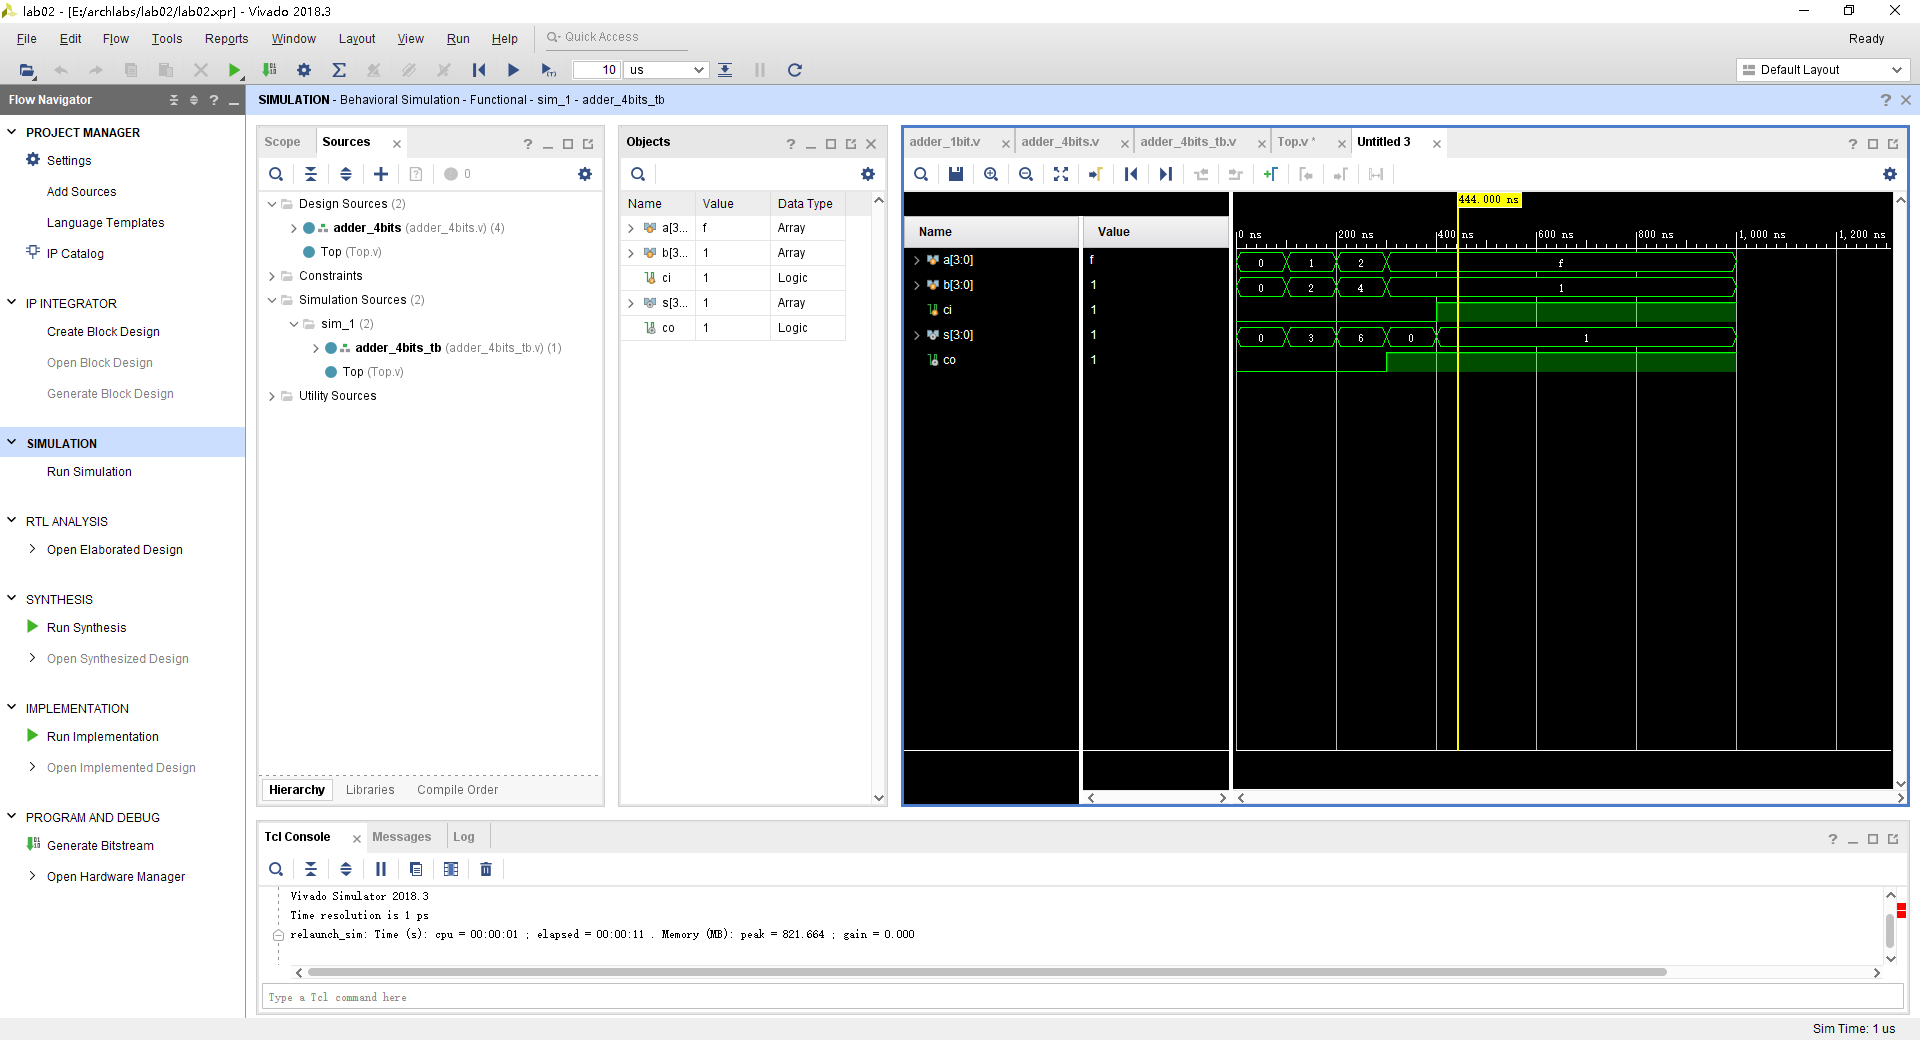
\includegraphics[scale=0.3]{../figure/02/lab02-1.PNG}
  \caption{实验结果1}\label{fig:1}
\end{figure}

\section{工程实现}

\subsection{顶层源文件}

将4位加法器的输出赋予LED和七段数码管显示,需要一个顶层源文件,命名为Top,代码如 </>CODE \ref{cd:4} 所示。

\begin{lstlisting}[language=verilog,caption={Top.v},label={cd:4}]
`timescale 1ns / 1ps

module Top(
    input clk_p,
    input clk_n,
    input [3:0] a,
    input [3:0] b,
    input reset,
    
    output led_clk,
    output led_do,
    output led_en,
    
    output wire seg_clk,
    output wire seg_en,
    output wire seg_do
    );
    wire CLK_i;
    wire Clk_25M;
    
    IBUFGDS IBUFGDS_inst (
        .O(CLK_i),
        .I(clk_p),
        .IB(clk_n)
    );
    
    wire [3:0] s;
    wire co;
    wire [4:0] sum;
    assign sum = {co, s};
    
    adder_4bits U1 (
    .a(a),
    .b(b),
    .ci(1'b0),
    .s(s),
    .co(co)
    );
    
    reg [1:0] clkdiv;
    always@(posedge CLK_i)
        clkdiv<=clkdiv+1;
    assign Clk_25M=clkdiv[1];
    
    display DISPLAY (
    .clk(Clk_25M),
    .rst(1'b0),
    .en(8'b00000011),
    .data({27'b0, sum}),
    .dot(8'b00000000),
    .led(~{11'b0, sum}),
    .led_clk(led_clk),
    .led_en(led_en),
    .led_do(led_do),
    .seg_clk(seg_clk),
    .seg_en(seg_en),
    .seg_do(seg_do)
    );
endmodule
\end{lstlisting}

Top.v 中用到了一个 display IP 核,需要添加该核,此处不赘述。

\subsection{管脚约束}

管脚约束文件为 lab02\_xdc.xdc,代码如 </>CODE \ref{cd:5} 所示。添加完管脚约束后即可下载验证。

\begin{lstlisting}[caption={lab02\_xdc.xdc},label={cd:5}]
  set_property PACKAGE_PIN W23 [get_ports {led[7]}]
  set_property PACKAGE_PIN AB26 [get_ports {led[6]}]
  set_property PACKAGE_PIN Y25 [get_ports {led[5]}]
  set_property PACKAGE_PIN AA23 [get_ports {led[4]}]
  set_property PACKAGE_PIN Y23 [get_ports {led[3]}]
  set_property PACKAGE_PIN Y22 [get_ports {led[2]}]
  set_property PACKAGE_PIN AE21 [get_ports {led[1]}]
  set_property PACKAGE_PIN AF24 [get_ports {led[0]}]
  set_property PACKAGE_PIN AC18 [get_ports clock_p]
  set_property PACKAGE_PIN W13 [get_ports reset]
  set_property IOSTANDARD LVCMOS33 [get_ports {led[7]}]
  set_property IOSTANDARD LVCMOS33 [get_ports {led[6]}]
  set_property IOSTANDARD LVCMOS33 [get_ports {led[5]}]
  set_property IOSTANDARD LVCMOS33 [get_ports {led[4]}]
  set_property IOSTANDARD LVCMOS33 [get_ports {led[3]}]
  set_property IOSTANDARD LVCMOS33 [get_ports {led[2]}]
  set_property IOSTANDARD LVCMOS33 [get_ports {led[1]}]
  set_property IOSTANDARD LVCMOS33 [get_ports {led[0]}]
  set_property IOSTANDARD LVDS [get_ports clock_p]
  set_property IOSTANDARD LVCMOS18 [get_ports reset]
\end{lstlisting}

\section{总结与反思}

经历过 lab01 的拷打后 lab02 做起来就轻松很多了。总的来说本次实验相当顺利,没有遇到什么困难。感谢老师和助教的指导!

\end{document}
